\documentclass[11pt]{article}
\usepackage[textwidth=18.0cm, textheight=23.0cm, top=2.0cm]{geometry}
\usepackage{pst-all}
\usepackage{amssymb}
\usepackage{tikz}
\usepackage{underscore}\begin{document}
\pagestyle{empty}


ClassName: \underline{\textbf{Class_04.2bp-18}}
\par
BinSize: \underline{\textbf{100 × 100}}
\par
ReduceSize: \underline{\textbf{100 × 100}}
\par
TypeNum: \underline{\textbf{39}}
\par
Num: \underline{\textbf{40}}
\par
OutS: \underline{\textbf{20000}}
\par
InS: \underline{\textbf{10710}}
\par
Rate: \underline{\textbf{0.536}}
\par
UB: \underline{\textbf{2}}
\par
LB0: \underline{\textbf{2}}
\par
LB: \underline{\textbf{2}}
\par
LBWithCut: \underline{\textbf{2}}
\par
NodeCut: \underline{\textbf{0}}
\par
ExtendedNodeCnt: \underline{\textbf{1}}
\par
GenNodeCnt: \underline{\textbf{1}}
\par
PrimalNode: \underline{\textbf{0}}
\par
ColumnCount: \underline{\textbf{2}}
\par
TotalCutCount: \underline{\textbf{0}}
\par
RootCutCount: \underline{\textbf{0}}
\par
LPSolverCnt: \underline{\textbf{1}}
\par
PricingSolverCnt: \underline{\textbf{0}}
\par
BranchAndBoundNum: \underline{\textbf{1}}
\par
isOpt: \underline{\textbf{true}}
\par
TimeOnInitSolution: \underline{\textbf{600.000 s}}
\par
TimeOnPrimal: \underline{\textbf{0.000 s}}
\par
TimeOnPricing: \underline{\textbf{0.000 s}}
\par
TimeOnRmp: \underline{\textbf{0.063 s}}
\par
TotalTime: \underline{\textbf{600.329 s}}
\par
\newpage


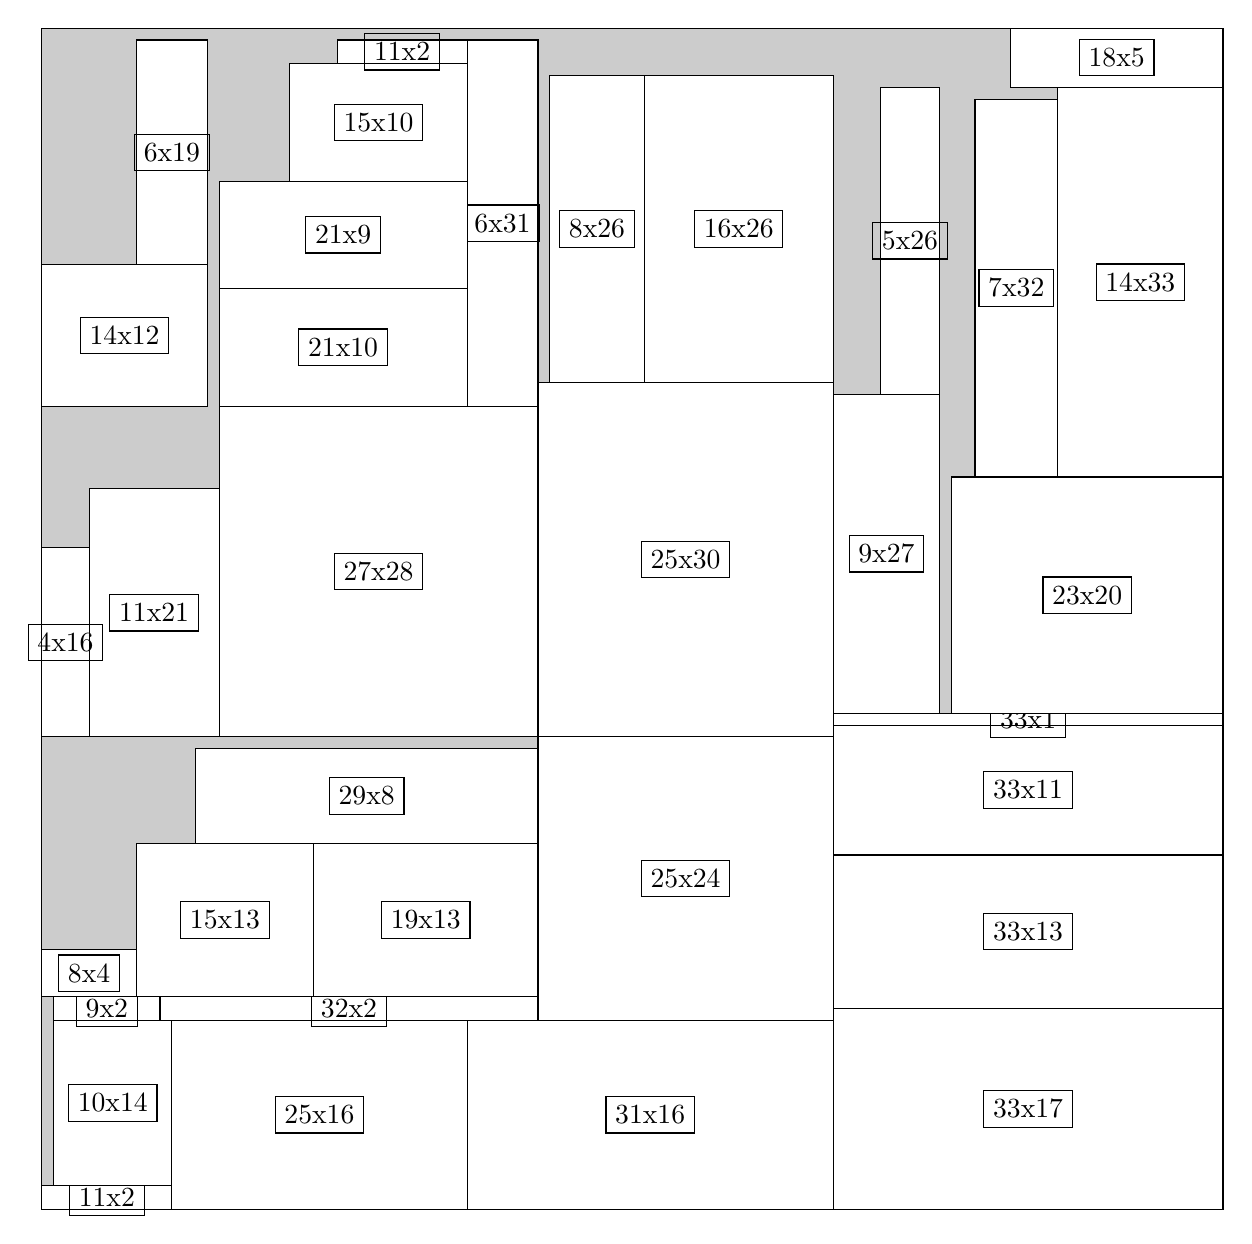
\begin{tikzpicture}[shorten >=1pt,scale=1.0,every node/.style={scale=1.0},->]
\tikzstyle{vertex}=[circle,fill=black!25,minimum size=14pt,inner sep=0pt]
\filldraw[fill=gray!40!white, draw=black] (0,0) rectangle (15.0,15.0);
\foreach \name/\x/\y/\w/\h in {33x17/10.049999999999999/0.0/4.95/2.55,33x13/10.049999999999999/2.55/4.95/1.95,33x11/10.049999999999999/4.5/4.95/1.65,33x1/10.049999999999999/6.1499999999999995/4.95/0.15,23x20/11.549999999999999/6.3/3.4499999999999997/3.0,14x33/12.9/9.299999999999999/2.1/4.95,7x32/11.85/9.299999999999999/1.05/4.8,9x27/10.049999999999999/6.3/1.3499999999999999/4.05,5x26/10.65/10.35/0.75/3.9,18x5/12.299999999999999/14.25/2.6999999999999997/0.75,31x16/5.3999999999999995/0.0/4.6499999999999995/2.4,25x16/1.65/0.0/3.75/2.4,11x2/0.0/0.0/1.65/0.3,10x14/0.15/0.3/1.5/2.1,25x24/6.3/2.4/3.75/3.5999999999999996,32x2/1.5/2.4/4.8/0.3,9x2/0.15/2.4/1.3499999999999999/0.3,19x13/3.4499999999999997/2.6999999999999997/2.85/1.95,15x13/1.2/2.6999999999999997/2.25/1.95,8x4/0.0/2.6999999999999997/1.2/0.6,29x8/1.95/4.6499999999999995/4.35/1.2,25x30/6.3/6.0/3.75/4.5,16x26/7.6499999999999995/10.5/2.4/3.9,8x26/6.45/10.5/1.2/3.9,27x28/2.25/6.0/4.05/4.2,11x21/0.6/6.0/1.65/3.15,4x16/0.0/6.0/0.6/2.4,6x31/5.3999999999999995/10.2/0.8999999999999999/4.6499999999999995,21x10/2.25/10.2/3.15/1.5,21x9/2.25/11.7/3.15/1.3499999999999999,15x10/3.15/13.049999999999999/2.25/1.5,11x2/3.75/14.549999999999999/1.65/0.3,14x12/0.0/10.2/2.1/1.7999999999999998,6x19/1.2/12.0/0.8999999999999999/2.85}
\filldraw[fill=white!40!white, draw=black] (\x,\y) rectangle node[draw] (\name) {\name} ++(\w,\h);
\end{tikzpicture}


w =33 , h =17 , x =67 , y =0 , v =561
\par
w =33 , h =13 , x =67 , y =17 , v =429
\par
w =33 , h =11 , x =67 , y =30 , v =363
\par
w =33 , h =1 , x =67 , y =41 , v =33
\par
w =23 , h =20 , x =77 , y =42 , v =460
\par
w =14 , h =33 , x =86 , y =62 , v =462
\par
w =7 , h =32 , x =79 , y =62 , v =224
\par
w =9 , h =27 , x =67 , y =42 , v =243
\par
w =5 , h =26 , x =71 , y =69 , v =130
\par
w =18 , h =5 , x =82 , y =95 , v =90
\par
w =31 , h =16 , x =36 , y =0 , v =496
\par
w =25 , h =16 , x =11 , y =0 , v =400
\par
w =11 , h =2 , x =0 , y =0 , v =22
\par
w =10 , h =14 , x =1 , y =2 , v =140
\par
w =25 , h =24 , x =42 , y =16 , v =600
\par
w =32 , h =2 , x =10 , y =16 , v =64
\par
w =9 , h =2 , x =1 , y =16 , v =18
\par
w =19 , h =13 , x =23 , y =18 , v =247
\par
w =15 , h =13 , x =8 , y =18 , v =195
\par
w =8 , h =4 , x =0 , y =18 , v =32
\par
w =29 , h =8 , x =13 , y =31 , v =232
\par
w =25 , h =30 , x =42 , y =40 , v =750
\par
w =16 , h =26 , x =51 , y =70 , v =416
\par
w =8 , h =26 , x =43 , y =70 , v =208
\par
w =27 , h =28 , x =15 , y =40 , v =756
\par
w =11 , h =21 , x =4 , y =40 , v =231
\par
w =4 , h =16 , x =0 , y =40 , v =64
\par
w =6 , h =31 , x =36 , y =68 , v =186
\par
w =21 , h =10 , x =15 , y =68 , v =210
\par
w =21 , h =9 , x =15 , y =78 , v =189
\par
w =15 , h =10 , x =21 , y =87 , v =150
\par
w =11 , h =2 , x =25 , y =97 , v =22
\par
w =14 , h =12 , x =0 , y =68 , v =168
\par
w =6 , h =19 , x =8 , y =80 , v =114
\par
\newpage


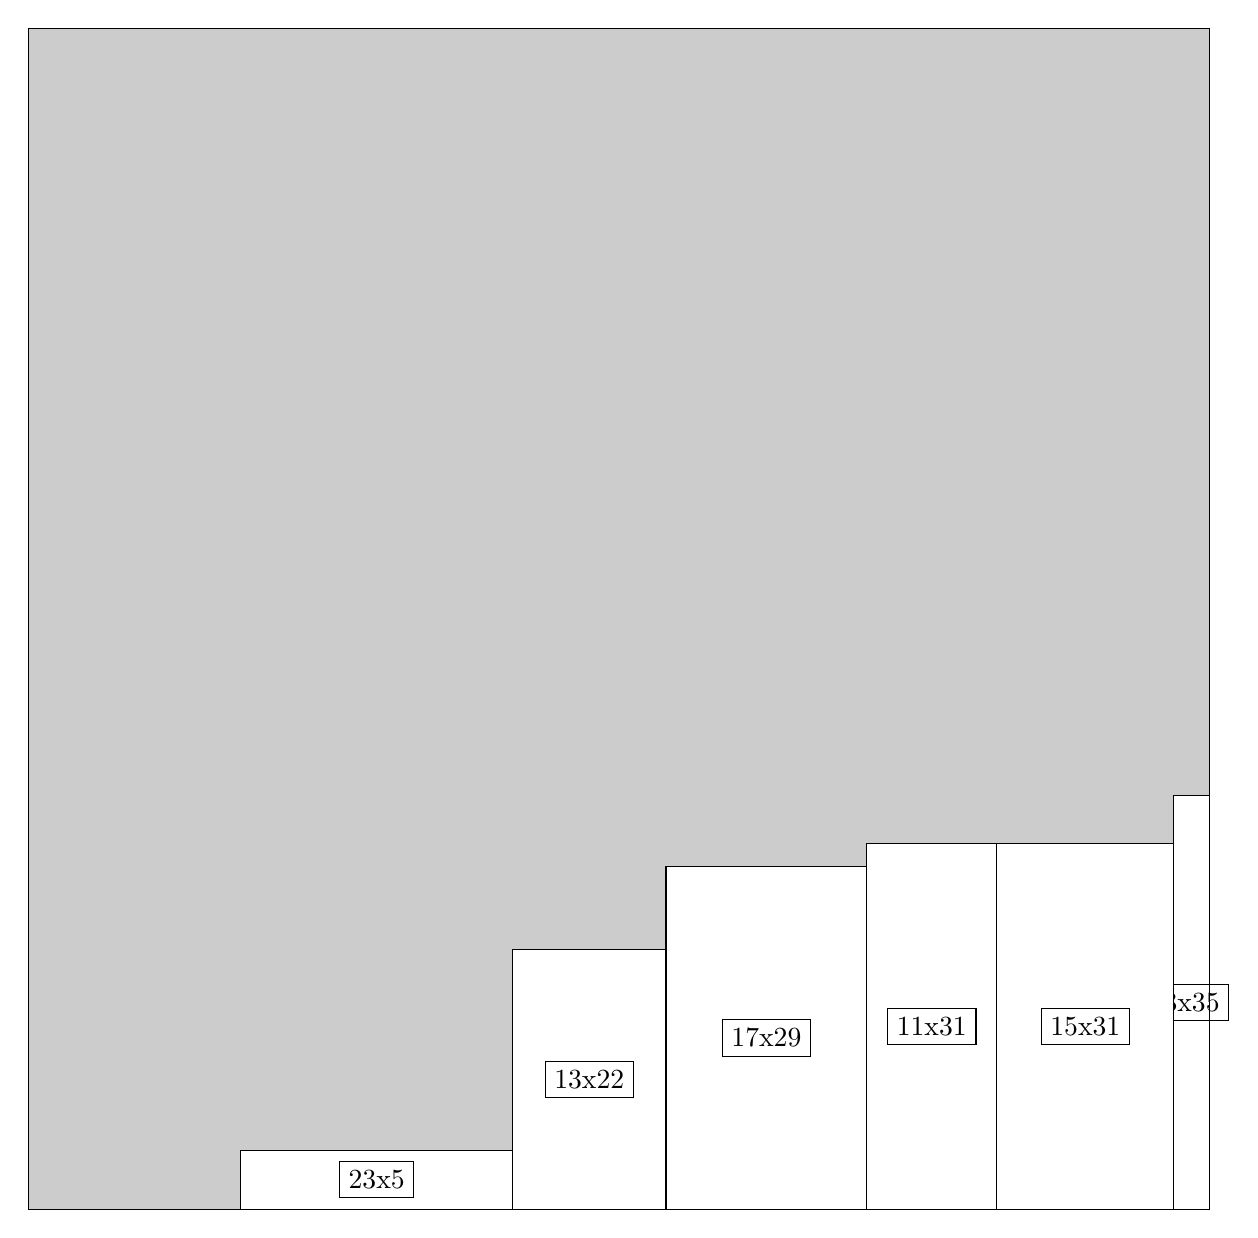
\begin{tikzpicture}[shorten >=1pt,scale=1.0,every node/.style={scale=1.0},->]
\tikzstyle{vertex}=[circle,fill=black!25,minimum size=14pt,inner sep=0pt]
\filldraw[fill=gray!40!white, draw=black] (0,0) rectangle (15.0,15.0);
\foreach \name/\x/\y/\w/\h in {3x35/14.549999999999999/0.0/0.44999999999999996/5.25,15x31/12.299999999999999/0.0/2.25/4.6499999999999995,11x31/10.65/0.0/1.65/4.6499999999999995,17x29/8.1/0.0/2.55/4.35,13x22/6.1499999999999995/0.0/1.95/3.3,23x5/2.6999999999999997/0.0/3.4499999999999997/0.75}
\filldraw[fill=white!40!white, draw=black] (\x,\y) rectangle node[draw] (\name) {\name} ++(\w,\h);
\end{tikzpicture}


w =3 , h =35 , x =97 , y =0 , v =105
\par
w =15 , h =31 , x =82 , y =0 , v =465
\par
w =11 , h =31 , x =71 , y =0 , v =341
\par
w =17 , h =29 , x =54 , y =0 , v =493
\par
w =13 , h =22 , x =41 , y =0 , v =286
\par
w =23 , h =5 , x =18 , y =0 , v =115
\par
\newpage


\end{document}